\documentclass[11pt]{article}
\usepackage[margin=1in]{geometry}
\usepackage{graphicx}
\usepackage{float}
\usepackage{xurl}
\usepackage[T1]{fontenc}
\usepackage{lmodern}
\usepackage{textcomp}
\usepackage[hidelinks]{hyperref}
\usepackage{caption}
\captionsetup{font=small}
\setlength{\parskip}{4pt}
\title{Overfitting or Overconfidence at the Data Wall?}
\author{Hanyu Yang\\Independent researcher}
\date{October 2026}
\graphicspath{{../figures/}}
\begin{document}
\maketitle

\begin{abstract}
\noindent As SOTA models hit the ``data wall,'' model developers are forced to train models on the same data multiple times. Scaling laws tell us this multi-epoch training comes with a penalty, but is the model actually getting worse, or just overconfident? To find out, we tested 125 public models (7M to 2.8B parameters, trained up to 64 epochs). We didn't retrain the models. We just used a quick mathematical adjustment to force them to second-guess their answers when tested on new documents. When we recalculated Lovelace et al.'s penalty for repeated data, it dropped by a third. For the models that actually started getting worse, half of that drop in quality was just overconfidence. The bottom line: repeating data does carry a real cost, but raw metrics exaggerate the damage.
\end{abstract}

\section*{Why this matters}
The standard scoring metric (loss) punishes a model for two things: making mistakes, and being arrogant about those mistakes. Our fix is a simple adjustment that only turns down the arrogance. It doesn't teach the model anything new. Because of this, if we apply our fix and the model's score improves, it proves that a chunk of the ``penalty'' wasn't actual brain-damage from repeating data---it was just the model being overly confident.

\section*{More repeats equal more arrogance (Figure 2)}
Models that only see data once are pretty realistic about their abilities. But as models repeat data, they get increasingly overconfident. For models trained across 16 to 64 epochs, their ``confidence dial'' had to be turned down significantly. The most extreme case was a 1.1-billion parameter model trained on the same data 59 times. It was so blindly certain of its answers that simply forcing it to second-guess itself improved its test score by a massive margin.

\setcounter{figure}{1}
\begin{figure}[H]
\centering
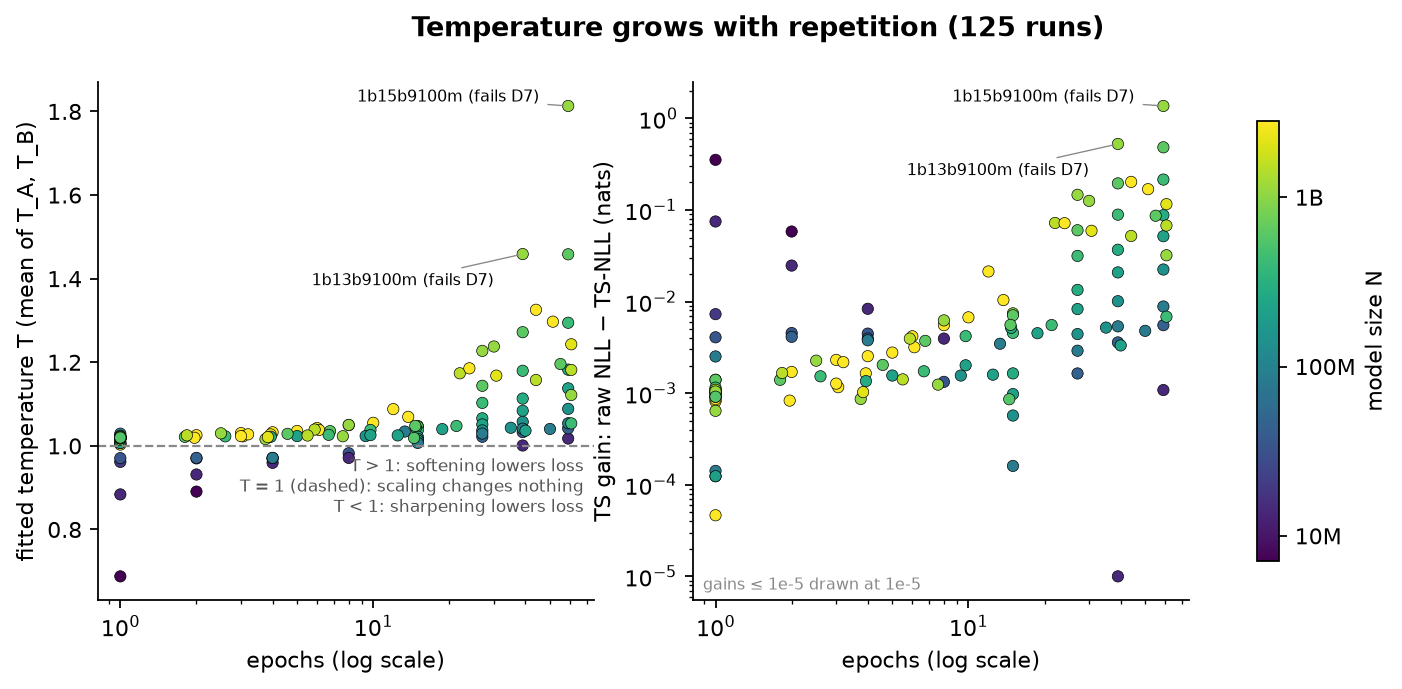
\includegraphics[width=0.9\linewidth]{fig2_temperature_vs_epochs.png}
\caption{Left: fitted temperature per run ($T > 1$ means softening the predicted probabilities lowers the loss). Right: how much loss one temperature removes. Colour is model size.}
\end{figure}

\section*{A third of the penalty is an illusion (Figures 3 and 5)}
Once we fixed the confidence levels across the board, the scaling law penalty dropped by about a third (leaving roughly 68\% of the penalty intact). We originally hoped the penalty would drop by at least half, but the data didn't support that. In fact, if you exclude a handful of models that completely broke during training, the real penalty is even higher (around 81\%). However, there is a silver lining: for the specific runs where a model's performance actually started getting worse over time, fixing the confidence cut that degradation right in half.

\begin{figure}[H]
\centering
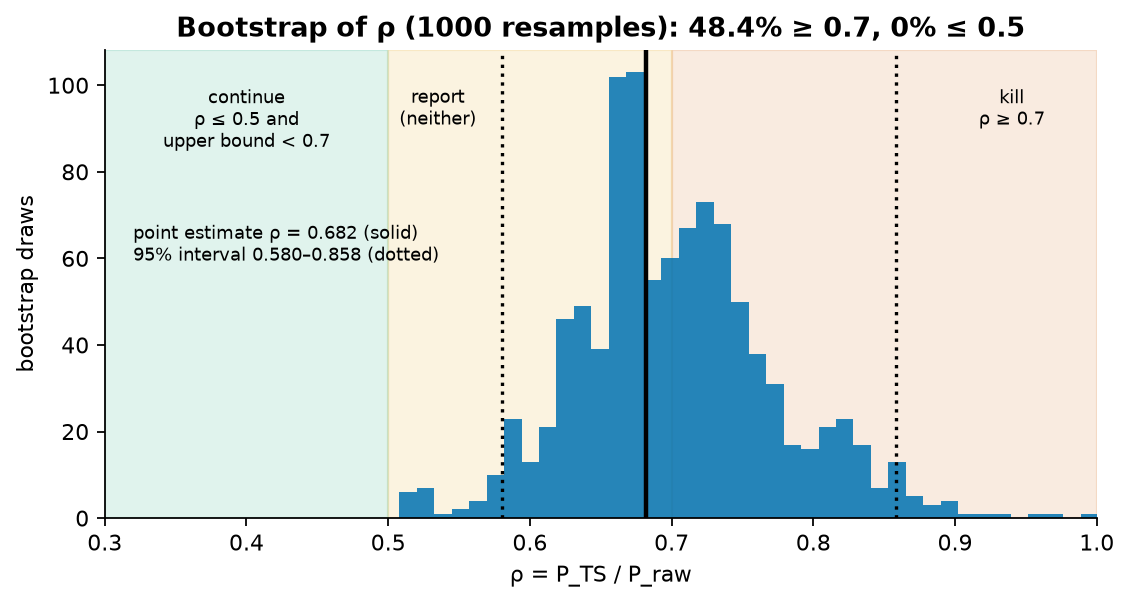
\includegraphics[width=0.75\linewidth]{fig3_rho_bootstrap.png}
\caption{Bootstrap distribution of $\rho$, the share of the penalty left after temperature scaling. Shading marks the point-estimate thresholds of the preregistered rule.}
\end{figure}

\setcounter{figure}{4}
\begin{figure}[H]
\centering
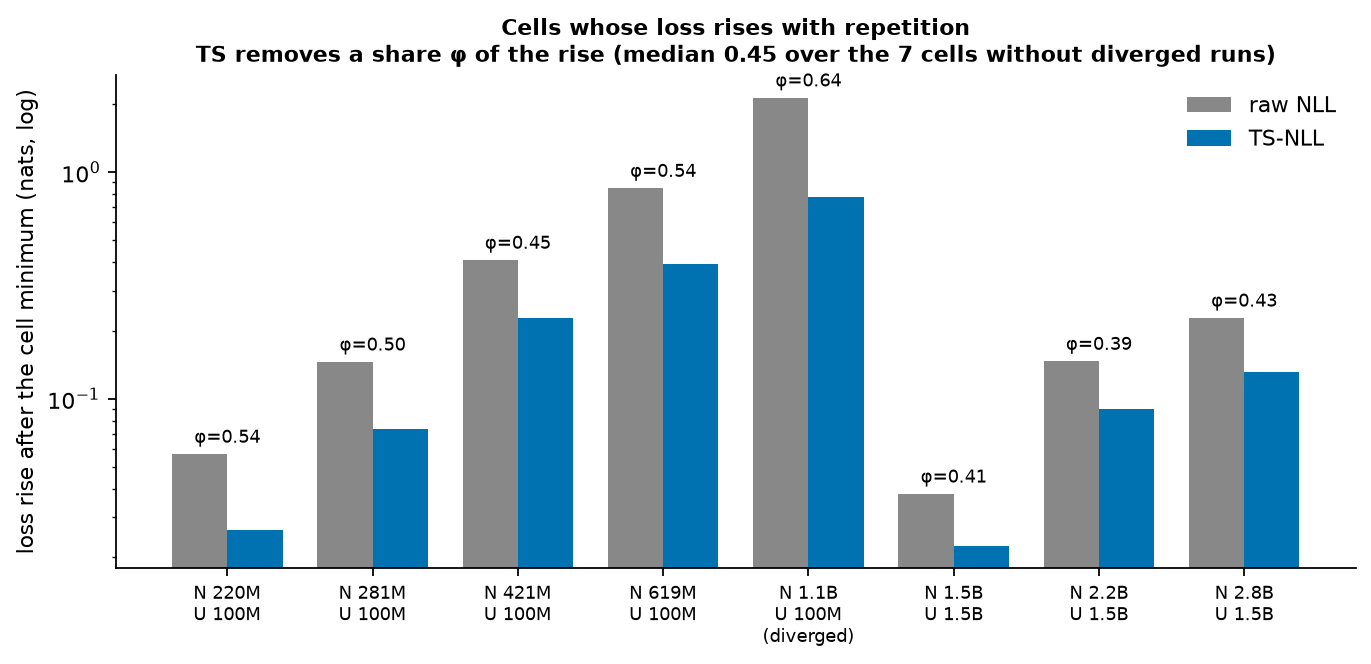
\includegraphics[width=0.9\linewidth]{fig5_post_minimum_rise.png}
\caption{For each (model size, unique data) cell whose loss rises after its minimum within 64 epochs: the rise in raw loss and in temperature-scaled loss, and the share that temperature removes.}
\end{figure}

\section*{The bottom line}
Training on the same data multiple times really does cause damage. But a significant chunk of what looks like ``overfitting'' is just the model getting too confident---and a quick mathematical tweak can fix it. You should check for this before trusting raw penalty scores.

Limits to keep in mind: We only tested models up to 2.8B parameters on the C4 dataset (the FineWeb models used in Lovelace et al.'s bigger penalty aren't public). Also, one of our pre-planned validation checks came in at 86\%, short of our strict 95\% target, so treat these findings as an exploratory first look.

Method, checks and code: \href{https://doi.org/10.5281/zenodo.23291816}{doi:10.5281/zenodo.23291816} $\cdot$ \url{https://github.com/SeverinVisionary/calrep}

\section*{References}
\small
\noindent[1] Muennighoff et al. Scaling Data-Constrained Language Models. NeurIPS 2023. arXiv:2305.16264. (Source of the 125 C4 checkpoints.)\\
{}[2] Lovelace et al. arXiv:2605.01640. (The overfitting penalty refit here.)

\section*{Use of AI tools}
The text of this note was written by the author. The analysis code, figures and the archive's documentation were produced with Claude Code (Anthropic), as described in the archive README.
\end{document}
